\documentclass[UTF8]{ctexrep}

\usepackage{graphicx}

\ctexset{
    section/name = {第,节},
    section/number = {\arabic{section}},
    subsection/number = {\arabic{section}.\arabic{subsection}}
}

\title{Aminer调研报告}
\author{王清雨}
% \usepackage{apacite}
\bibliographystyle{acm}

\begin{document}

\maketitle
\newpage
\part{历史}
\section{aminer发展历史}

\paragraph{2006年6月}
信息提取,学者、论文、会议搜索
\paragraph{2006年8月}
重写上述功能
\paragraph{2007年7月}
添加学者研究兴趣、关联搜索(\textbf{\textit{association search}})、\textbf{\textit{survey search}}?
\paragraph{2008年4月}
查询理解(\textbf{\textit{Query understanding}})、新的搜索界面、日志分析
\paragraph{2008年11月}
图搜索、主题挖掘(\textbf{\textit{topic mining}})
\paragraph{2009年4月}
信息编辑、开放资源
\paragraph{2009年12月}
学术统计数据(\textbf{\textit{Academic statistics}})、用户反馈、精细化排名

\section{论文发表历史}

\subsection{社交网络分析}
\textbf{\textit{Topic-based} social influence analysis in large-scale networks}

%--------------------------%

\paragraph{2009年}
\subparagraph{Social influence analysis in large-scale networks}~\cite{tang2009social}
\par 主要研究社交网络\textbf{\textit{(social network)}}的建模、分类及其内部关系,提出了\textbf{Topical Affinity Propagation}用来对社交网络进行建模。最终能够找到一个topic下最具代表性的节点,同时发现节点对周围节点的影响。
\par 有很多看不懂的机器学习的公式和算法

\subparagraph{Topic distributions over links on web}~\cite{tang2009topic}
\par 主要研究如何对网页上的链接进行分类和如何量化链接的影响力
\par 接下来就看不懂了

\begin{figure}[h]
    \caption{topical factor graph model}
    \centering
    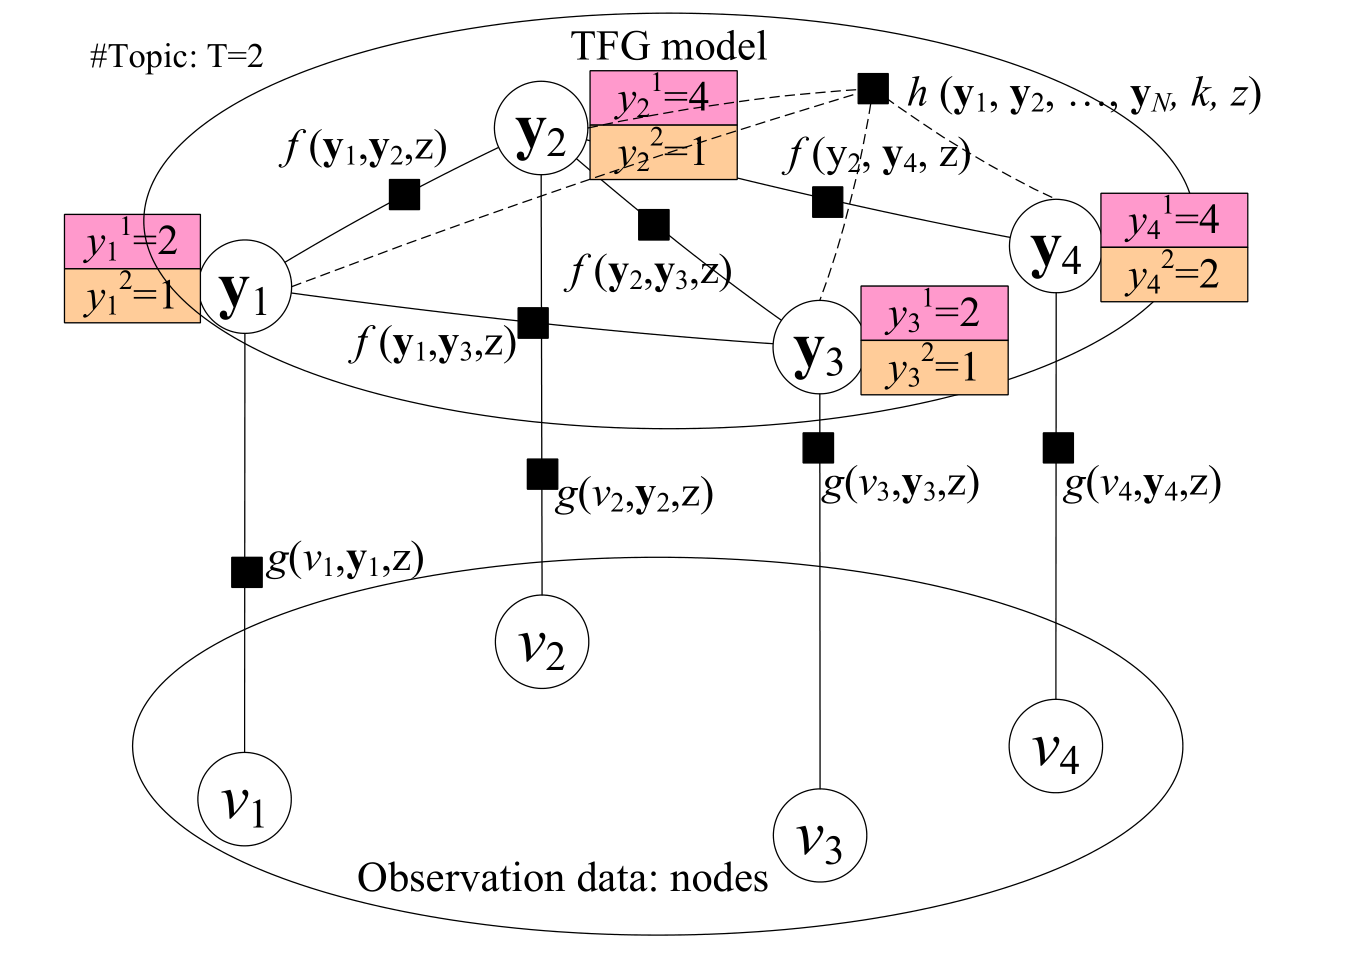
\includegraphics[width=0.8\textwidth]{assets/figures/model1.png}
    \label{fig:model1}
\end{figure}
%--------------------------%

\paragraph{2010年}
\subparagraph{Mining Advisor-Advisee Relationships from Research
Publication Networks}\cite{wang2010mining}
\par 主要研究如何将导师、学生关系从合作关系中提取、挖掘出来,并给出一种学习方法,用来提升提取的效果。

\par 可见这是如今\texttt{aminer}\footnote{https://www.aminer.cn}所做的事情的简化版。
\par {\heiti 关键词:}\emph{relationship mining, time-constrained probabilistic factor graph model, jointly likelihood objective function, advisor-advisee prediction}


\subparagraph{Social community analysis via a factor graph model}~\cite{yang2010social}
\par 与\cite{tang2009topic}基本相同

\subparagraph{Social community analysis via a factor graph model}~\cite{tan2010social}
\par 与\cite{tang2009topic,yang2010social}基本相同


%--------------------------%

\subsection{社交网络排名}
\textbf{Topic-based heterogeneous ranking}

\paragraph{2008年}
\subparagraph{A Topic Modeling Approach and its Integration into the Random Walk
Framework for Academic Search}~\cite{tang2008topic}
\par 建立了一种新的建模方式\textit{Author-Conference-Topic(ACT) model},能够同时对论文、作者、出版物进行建模,还采用\textit{Random walk framework}来加强排名\textit{ranking}

\subparagraph{ArnetMiner: Extraction and Mining
of Academic Social Networks}\cite{tang2008arnetminer}
\par 应该是\texttt{aminer}\footnote{https://www.aminer.cn}系统第一次在唐杰老师的论文中正式发布\textit{(之前都是作为一个测试系统有提到)},开篇就提到了\texttt{aminer}的目的及其解决
\begin{itemize}
    \item 自动从互联网获取学者信息\quad \texttt{=>} \quad \textit{uniyied tagging approach}
    \item 将获取到的信息整合入现有数据库的网络中(不同来源的信息如何统一)
    \item 对整个学术网络进行建模\quad \texttt{=>} \quad \textit{ACT model}
    \item 为学术网络提供搜索服务
\end{itemize}
\par 同时,文章里也提到他们使用一个概率框架\textbf{\textit{a probabilistic
framework}}来解决重名问题\textit{(name ambiguity problem)},还提到了\cite{tang2008topic}中所提出的同时对文章的多种信息进行建模的方法。
\par 有关架构方面的内容见下文第二部分。
\par 有关相关技术的内容间下文第四部分。

%--------------------------%

\subsection{知识获取}
\textbf{Acquiring knowledge from social Web}

\paragraph{2006年}
\subparagraph{Tree-Structured Conditional Random Fields for
Semantic Annotation}~\cite{tang2006tree}


\paragraph{2007年}
\subparagraph{Social network extraction of academic researchers}~\cite{tang2007social}


\paragraph{2010年}
\subparagraph{A combination approach to web user profiling}~\cite{tang2010combination}


\subsection{重名问题}
\textbf{name disambiguation}

\paragraph{2007年}
\subparagraph{A constraint-based probabilistic framework for name disambiguation}~\cite{zhang2007constraint}


\paragraph{2010年}
\subparagraph{A unified probabilistic framework for name disambiguation in digital library}~\cite{tang2011unified}


\paragraph{2011年}
\subparagraph{Adana: Active name disambiguation}~\cite{wang2011adana}


\paragraph{2018年}
\subparagraph{Name Disambiguation in AMiner: Clustering, Maintenance, and Human in the Loop.}~\cite{zhang2018name}


\part{组织结构}

从\cite{tang2008arnetminer}中可以看到如下图所示的架构,主要有以下几部分组成:
\begin{itemize}
    \item {\heiti 获取信息}\textit{Extraction}
    \item {\heiti 整合}\textit{Integration}
    \item {\heiti 存储与访问}\textit{Storage and Access}
    \item {\heiti 建模}\textit{Modeling}
    \item {\heiti 搜索}\textit{Search Services}
\end{itemize}
\begin{figure}[h]
    \caption{topical factor graph model}
    \centering
    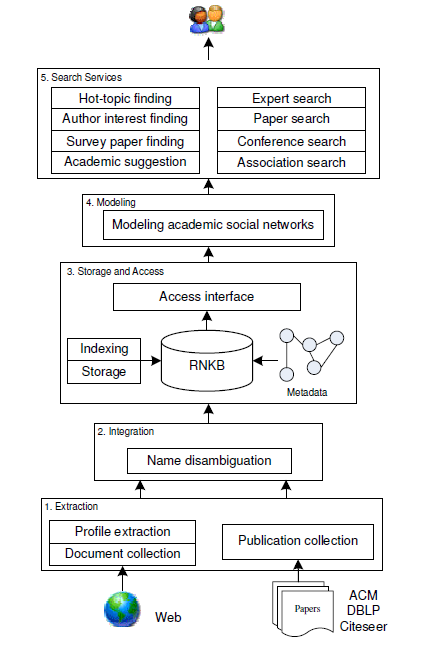
\includegraphics[width=0.6\textwidth]{assets/figures/arch.PNG}
    \label{fig:arch}
\end{figure}

\section{aminer遇到的挑战}

\paragraph{获取信息} 鉴于原来对数据的爬取都是基于特定的数据集,是否存在一种通用的爬虫,能够适用于所有的网页(个人认为不太行)

\paragraph{整合} 如何充分利用我们已有的信息来解决重名问题\textbf{\textit{(disambiguation)}}

\paragraph{建模} 之前没有一种同时对各种信息进行建模的方式,并且不同的建模方式之间有着较大的区别,应当研究那种建模方式最适合学术搜索\textbf{\textit{(academic search)}}

\par 其余的部分aminer采用了传统的方式。




\part{特点}

\part{后台技术}
后台技术主要根据组织结构从四个方面来说:数据获取、重名问题、建模以及搜索。

\section{数据获取}
相关论文:\cite{tang2008arnetminer}
数据获取分为两个部分,\textbf{处理}和\textbf{CRF model}

\paragraph{处理}\textit{Process}
\par 处理分为三步:
\begin{itemize}
    \item 有关页面识别
    \item 处理
    \item 提取
\end{itemize}
\subparagraph{有关页面识别}先通过搜索引擎获取到一系列网页,然后通过二分类分类器\textit{binary classifier}识别其中的学者主页。分类器采用支持向量机\textit{Support Vector Machines}作为分类模型。
\subparagraph{处理}先将文字划分为\textit{token},再给它们打上标签,每个标签对应一种学者的一个\textit{property}
\subparagraph{提取}从打好标签的数据中提取出需要的信息


\section{重名问题\textit{Name Disambiguation}}
相关论文:\cite{tang2008arnetminer}

没太看懂

\section{建模}
相关论文:\cite{tang2008arnetminer,tang2008topic}

没太看懂

\section{搜索}
相关论文:\cite{tang2008arnetminer,zhang2007constraint,tang2011unified,wang2011adana,zhang2018name}

\bibliography{papers}
\end{document}
